\section{A Common-Source Amplifier}

\subsection{Experiment Design}
    \subsubsection{Background}


    \subsubsection{Propose}
    \begin{itemize}
        \item 2N7000 MOSEFT
        \item Resistors
        \item Breadboard
        \item Oscilloscope
        \item Function Generator
        \item DC Power Supply
    \end{itemize}

\subsection{Experiment Design}
    \subsubsection{Materials}
        In this experiment, we will use the following components:
        \begin{itemize}
            \item To measure the quiescent-point of a common-source amplifier
            \item To evaluate the small-signal amplification function of a common-source amplifier
        \end{itemize}

    \subsubsection{Circuit Diagram}
        The following circuit diagrams 
        \begin{figure}[H]
            \centering
                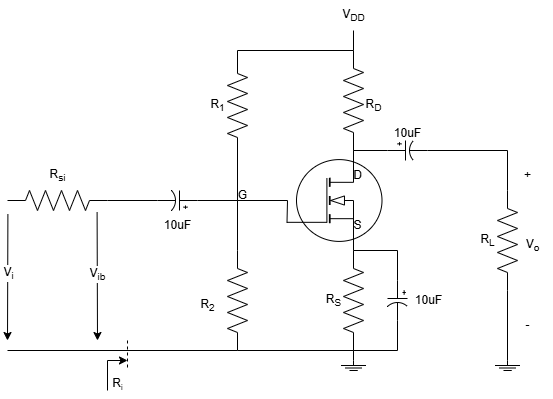
\includegraphics[width=1\linewidth]{Experiment_09/Circuit/Lab9.drawio.png}
                \caption{Common-Source Amplifier Circuit}
                \label{cir:9}
        \end{figure}

    \subsubsection{Theoretical Analysis}
        \begin{enumerate}[a]
            \item \textbf{DC Analysis}\par
                \begin{figure}[H]
                    \centering
                        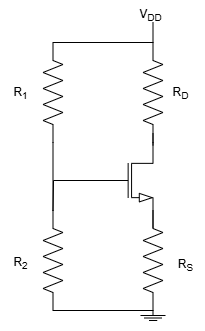
\includegraphics[width=0.3\linewidth]{Experiment_09/Circuit/L9DC.drawio.png}
                        \caption{DC equvlent Circuit}
                        \label{cir:9DC}
                \end{figure}
            \item \textbf{AC Analysis}\par
                \begin{figure}[H]
                    \centering
                        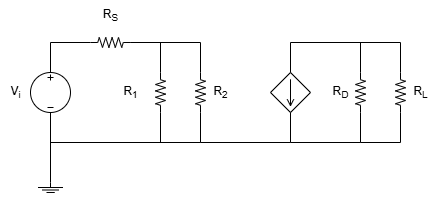
\includegraphics[width=0.3\linewidth]{Experiment_09/Circuit/L9AC.drawio.png}
                        \caption{AC equvlent Circuit}
                        \label{cir:9AC}
                \end{figure}
        \end{enumerate}

\subsection{Experiment record}
    \subsubsection{Voltage gain}
    We recorded the following data to calculate voltage gain of the common-source amplifier:
    \begin{table}[h]
        \centering
        \begin{tabular}{l|rrrr}
            Vib   & 0.0646 & 0.052 & 0.039 & 0.025 \\
            Vo    & 0.51  & 0.413 & 0.309 & 0.205 \\
            \midrule
            A     & 7.894737 & 7.942308 & 7.923077 & 8.2 \\
            \end{tabular}%
        \caption{Voltage gain}
    \end{table}
    The voltage gain is calculated with the formula: $\frac{V_O}{V_I}$

    \subsubsection{Input impedance}
    \begin{table}[h]
        \centering
    \begin{tabular}{lr}
        Vib   & 0.066 \\
        Vi    & 0.072 \\
        \end{tabular}%
        \caption{Input impedance}
    \end{table}
    And the input impedance is calculated as:
        
    \subsubsection{Output impedance}
    To calculate the output impedance, we recorded the following data:
    \begin{table}[h]
        \centering
    \begin{tabular}{lcc}
        AC OR & RL = 300k & RL = 1k \\
        Vi    & 0.073 & 0.0.73 \\
        Vo    & 0.522 & 0.436 \\
        \end{tabular}%
        \caption{Output impedance}
    \end{table}

\subsection{Experiment Conclusion}
    \subsubsection{Conclusion}
    This experiment presents us the common-source MOSFET amplifier. The experiment reinforces my understanding of the MOSFET circuit.\par